% This is samplepaper.tex, a sample chapter demonstrating the
% LLNCS macro package for Springer Computer Science proceedings;
% Version 2.20 of 2017/10/04
%
\documentclass[runningheads]{llncs}
%
\usepackage{graphicx}
% Used for displaying a sample figure. If possible, figure files should
% be included in EPS format.
\usepackage{tikz}
\usetikzlibrary{arrows}
\usepackage{verbatim}
\usepackage{algorithm}
\usepackage[noend]{algpseudocode}
\usepackage{amssymb}
\usepackage{amsfonts}
\usepackage{amsmath}
\let\proof\relax\let\endproof\relax
\usepackage{amsthm}
\usepackage{graphicx}
%\usepackage[all]{xy}
\usepackage{array}
\usepackage{enumitem}
%\usepackage{cite}
\usepackage[numbers,sectionbib]{natbib}
\usepackage{wrapfig}
\theoremstyle{definition}
\renewcommand{\qedsymbol}{\hfill\ensuremath{\blacksquare}}
%\newtheorem{definition}{Definition}[section]
% If you use the hyperref package, please uncomment the following line
% to display URLs in blue roman font according to Springer's eBook style:
% \renewcommand\UrlFont{\color{blue}\rmfamily}
\usepackage[breaklinks=true]{hyperref}
\usepackage{breakcites}
\renewcommand\UrlFont{\color{blue}\rmfamily}

\input{lib/coq-listings}

%%% added lib and commands
\newcommand{\squash}{\itemsep=0pt\parskip=0pt}
\input{prelude.tex}
\usepackage{varwidth}
%\usepackage{minted}
%\usepackage{tcolorbox}
\usepackage{caption}

\newcolumntype{M}[1]{>{\centering\arraybackslash}m{#1}}
\newcolumntype{N}{@{}m{0pt}@{}}

\begin{document}
%
\title{An Ordering over Attestation Protocols\thanks{Supported by organization x.}}
%
%\titlerunning{Abbreviated paper title}
% If the paper title is too long for the running head, you can set
% an abbreviated paper title here
%
\author{Anna Fritz \and
Sarah Johnson \and
Perry Alexander}
%
\authorrunning{F. Author et al.}
% First names are abbreviated in the running head.
% If there are more than two authors, 'et al.' is used.
%
\institute{Institute for Information Sciences \\ The
  University of Kansas \\ Lawrence, KS 66045 \\
  \email{\{arfritzz,sarahjohnson,palexand\}@ku.edu}}
%
\maketitle              % typeset the header of the contribution
%
\begin{abstract}
The abstract should briefly summarize the contents of the paper in
15--250 words.

\keywords{First keyword  \and Second keyword \and Another keyword.}
\end{abstract}
%
%
%
\section{Introduction}
A key facet of the negotiation routine is attestation protocol selection where selecting the best attestation protocol from among many poses a challenging problem. This difficulty can be attributed to situational nuances that impact an ordering and the variety of attestation scenarios that exist. To further complicate the problem, various dimensions for protocol analysis arise such as a protocol's complexity, its resource consumption, or its vulnerability to an adversary. Considering all facets at once makes the ordering problem exponentially harder. We therefore simplify the problem by focusing solely on comparing protocols based on their susceptibility to attack. Towards this goal, we introduce equivalence and partial order relations over Copland attestation protocols where a better protocol increases the minimal work required of an active adversary to thwart an appraiser. Our formally-modeled, Coq-based solution includes verified properties of the adversary-constrained ordering relations. Furthermore, we apply our ordering scheme to representative examples to demonstrate its accuracy and efficacy.

This emerging adversary-constrained protocol ordering requires a few key assumptions and definitions. First, we consider an active adversary that is capable of corrupting any component of the target system causing it to deviate from its regular behavior and is also capable of repairing any component of the target system returning it to its regular state. We assume that the target system has a special component, namely a root of trust for measurement (RTM), that cannot be attacked by the adversary. Furthermore, we assume an adversary will always choose the easiest attack to thwart an appraiser. Therefore, a better protocol increases the demands of an active adversary by making the easiest attack more difficult. For an adversary to attack an attestation protocol means to corrupt and repair a target system's components in a way that passes appraisal and therefore evades detection at the final measurement event. A corrupt measurer---either a measurer that itself is in a corrupt state or a measurer that relies on some other component that is in a corrupt state---will always generate evidence that indicates its target is in its regular state. While a regular measurer will generate evidence that accurately reflects the corruption state of its target. Our analysis relies solely on the structure of possible attacks and is agnostic to the specific details of how an adversary can corrupt or repair system components as required by an attack.

Considering these assumptions, the formalized model and subsequent analysis reveal the following two principles.

\begin{enumerate}
    %\squash
    \item Increasing the number of measurement events does not necessarily further confine the adversary 
    \item Measurements that mimic the system's dependency chain better confine the adversary
\end{enumerate}

% \noindent Contrary to what may seem intuitive, increasing the volume of measurement operations may not place additional constraints on an active adversary. That is, additional measurements do not necessarily result in additional adversary actions therefore not always affecting the  trustworthiness of evidence. Rather, we prove measuring closer to the root of trust with a protocol that mimics the system's dependencies verifiably makes an adversary's weakest attacks more difficult. Rowe set out to understand this idea by stating that a well-supported measurement chain, one that includes components and their dependencies up to a root of trust, is more difficult for an adversary to corrupt \cite{Rowe:2016:Confining}. We formally model and demonstrate this hypothesis, mechanically proving that selecting well-supported measurements during negotiation better constrains an adversary.


\section{Preliminaries}

Properties of orderings and the Chase model finder developed by MITRE \cite{Ramsdell:2020:Chase} are paramount tools for our adversary-constrained protocol ordering and subsequent analysis. Key concepts include equivalence and partial order relations as well as Chase generated attack trees. 

\subsection*{Properties of Orders}

Critical to our study is various properties of a binary relation $R$ on a set $X$. We specifically consider the following properties, formally defined below.

\begin{itemize}
    \squash
    \item \emph{reflexive} -- $ \forall\: x\: \in X$, $R\: x\: x$
    \item \emph{irreflexive} -- $ \forall \: x\: \in X, \: \neg \: R\: x\: x$
    \item \emph{symmetric} -- $ \forall\: x\: , y\: \in X,$ $R\: x\: y\:\rightarrow R\: y\: x$
    \item \emph{asymmetric} --  $\forall\: x,\: y\:\in X,\: R\: x\: y\:\: \rightarrow  \:\: \neg \:R\: y\: x $  
    \item \emph{antisymmetric} --  $\forall\: x,\: y\:\in X,\: R\: x\: y\:\: \rightarrow \:\: R\: y\: x \rightarrow \:x = y$ 
    \item \emph{transitive} -- $ \forall\: x,\: y,\: z\:\in X$, $R\: x\: y\: \rightarrow R\: y\: z \rightarrow R\: x\: z$
\end{itemize}

\noindent Combining these properties in specific ways lends itself to the following ordering relations.

\begin{itemize}
    \squash
    \item a \emph{preorder} is reflexive and transitive
    \item an \emph{equivalence} relation is reflexive, symmetric, and transitive 
    \item a \emph{partial order} is reflexive, antisymmetric, and transitive 
    \item a \emph{strict partial order} is irreflexive, asymmetric, and transitive 
\end{itemize}

\noindent When attempting to introduce new ordering relations, as with this protocol ordering, each required property must be proven.  

\subsection*{Chase Analysis}

Chase \cite{Ramsdell:2020:Chase,Rowe:2021:AutomatedTrust} is a first order model finder that utilizes geometric logic\cite{Enderton:logic} to find minimal models of a given theory. Inputs to the Chase model finder include axiomatized queries describing assumptions and system dependencies. From those queries, Chase generates all models which satisfy the given formulas. 

Chase can be leveraged to understand the susceptibility of a Copland protocol to attack \cite{Rowe:2021:AutomatedTrust}. Given a Copland phrase, a model of Copland adversary events, and a model of the evaluated protocol, Chase produces output containing all possible protocol executions rendered in \texttt{.xhtml} as attack trees. These sequential attack trees \cite{Horne:Attack, Jhaware:attack} are formal models of all the ways in which an adversary might attack a system while evading detection by the attestation. Within the attack trees, the presence of an active adversary can be recognized by the corruption and repair of various components in the target system. The specific details of how an adversary performs these corruption and repairs are not the focus of this work nor of Chase. Instead, the goal of Chase for protocol analysis is to produce easily identifiable corruption and repair events, allowing users to better understand potential vulnerabilities within the system and Copland protocol. 

Consider an example protocol where two measurements are performed in sequence as abstractly rendered below.

\begin{center}
    *target: $@_{\texttt{p1}}$[\texttt{ms1 +<+} $\at{\texttt{p1}}{\texttt{ms2}}]$
\end{center}

\noindent At place \texttt{p1}, the measurement \texttt{ms1} is performed followed by, at place \texttt{p1} again, the final measurement \texttt{ms2}. We assert that \texttt{ms1} and \texttt{ms2} depend on some components of the environment, namely \texttt{c1} and \texttt{c2}; additionally \texttt{ms1} depends on \texttt{c3}. These system dependencies are realized within the user-defined theory file input into the Chase model finder. Running Chase on this protocol generates attack trees as found in Figure \ref{fig:chase-ex}. In these figures, the prefix \texttt{ms} represents measurement events and are presented within green boxes. The prefix \texttt{c\_} represents corruption events and the prefix \texttt{r\_} represents repair events. Both corruption and repair events are classified as adversary events and are presented within yellow and orange boxes respectively. This abstract labeling scheme mirrors that of the Chase output.

\begin{figure}[hbtp]
    \centering 
    \begin{tabular}{c c c}
        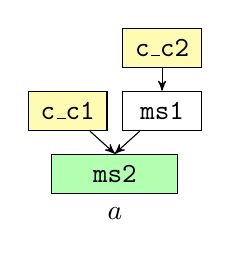
\begin{tikzpicture}[->,>=stealth']

    \node[rectangle,
          draw,
          fill = green!30,
          minimum width = 1.6cm, 
          minimum height = 0.5cm
          ] (ms4) at (0,0) {};
    \node[] at (ms4.center) {\texttt{ms2}};

    \node[rectangle,
        draw,
        minimum width = 1cm, 
        minimum height = 0.5cm
        ] (ms2) at (.6,.8) {};
    \node[] at (ms2.center) {\texttt{ms1}};


    \node[rectangle,
        draw,
        fill = yellow!30,
        minimum width = 1cm, 
        minimum height = 0.5cm
        ] (sys) at (-.6,.8) {};
    \node[] at (sys.center) {\texttt{c\_c1}};

    \node[rectangle,
        draw,
        fill = yellow!30,
        minimum width = 1cm, 
        minimum height = 0.5cm
        ] (vc) at (.6,1.6) {};
    \node[] at (vc.center) {\texttt{c\_c2}};

    \node[rectangle,
        minimum width = 1cm, 
        minimum height = 0.5cm
        ] (label) at (0,-.5) {};
    \node[] at (label.center) {$a$};


    \path[every node/.style={font=\sffamily\small}]
    %host1 path
    (vc) edge [] node [right] {} (ms2.north) 
    (sys) edge [] node [right] {} (ms4.north)
    (ms2) edge [] node [right] {} (ms4.north) ;


\end{tikzpicture} & 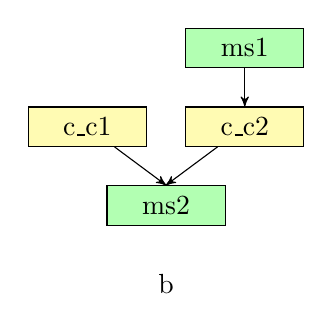
\begin{tikzpicture}[->,>=stealth']

    \node[rectangle,
          draw,
          fill = green!30,
          minimum width = 1.5cm, 
          minimum height = 0.5cm
          ] (ms4) at (0,0) {};
    \node[] at (ms4.center) {ms2};

    \node[rectangle,
        draw,
        fill = green!30,
        minimum width = 1.5cm, 
        minimum height = 0.5cm
        ] (ms2) at (1,2) {};
    \node[] at (ms2.center) {ms1};


    \node[rectangle,
        draw,
        fill = yellow!30,
        minimum width = 1.5cm, 
        minimum height = 0.5cm
        ] (sys) at (-1,1) {};
    \node[] at (sys.center) {c\_c1};

    \node[rectangle,
        draw,
        fill = yellow!30,
        minimum width = 1.5cm, 
        minimum height = 0.5cm
        ] (vc) at (1,1) {};
    \node[] at (vc.center) {c\_c2};

    \node[rectangle,
        minimum width = 1cm, 
        minimum height = 0.5cm
        ] (label) at (0,-1) {};
    \node[] at (label.center) {b};


    \path[every node/.style={font=\sffamily\small}]
    %host1 path
    (vc) edge [] node [right] {} (ms4.north) 
    (sys) edge [] node [right] {} (ms4.north)
    (ms2) edge [] node [right] {} (vc.north) ;


\end{tikzpicture} & 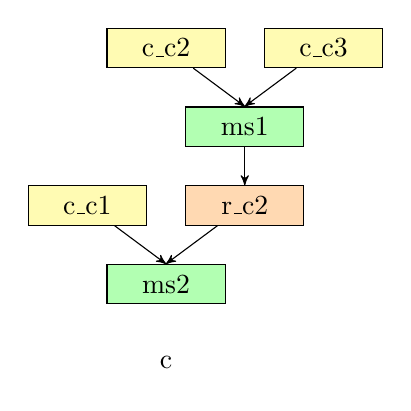
\begin{tikzpicture}[->,>=stealth']

    \node[rectangle,
          draw,
          fill = green!30,
          minimum width = 1.5cm, 
          minimum height = 0.5cm
          ] (ms4) at (0,-1) {};
    \node[] at (ms4.center) {ms2};

    \node[rectangle,
        draw,
        fill = green!30,
        minimum width = 1.5cm, 
        minimum height = 0.5cm
        ] (ms2) at (1,1) {};
    \node[] at (ms2.center) {ms1};


    \node[rectangle,
        draw,
        fill = yellow!30,
        minimum width = 1.5cm, 
        minimum height = 0.5cm
        ] (sys) at (-1,0) {};
    \node[] at (sys.center) {c\_c1};

    \node[rectangle,
        draw,
        fill = yellow!30,
        minimum width = 1.5cm, 
        minimum height = 0.5cm
        ] (c2) at (0,2) {};
    \node[] at (c2.center) {c\_c2};

    \node[rectangle,
        draw,
        fill = yellow!30,
        minimum width = 1.5cm, 
        minimum height = 0.5cm
        ] (vc) at (2,2) {};
    \node[] at (vc.center) {c\_c3};

    \node[rectangle,
        draw,
        fill = orange!30,
        minimum width = 1.5cm, 
        minimum height = 0.5cm
        ] (r1) at (1,0) {};
    \node[] at (r1.center) {r\_c2};

    \node[rectangle,
        minimum width = 1cm, 
        minimum height = 0.5cm
        ] (label) at (0,-2) {};
    \node[] at (label.center) {c};


    \path[every node/.style={font=\sffamily\small}]
    %host1 path
    (r1) edge [] node [right] {} (ms4.north) 
    (c2) edge [] node [right] {} (ms2.north) 
    (vc) edge [] node [right] {} (ms2.north) 
    (sys) edge [] node [right] {} (ms4.north)
    (ms2) edge [] node [right] {} (r1.north) ;


\end{tikzpicture} 
    \end{tabular}
    \caption[Example Chase Models]{Example Chase models}
    \label{fig:chase-ex}
\end{figure}




\section{Overview}
We introduce a Coq-based, formally-verified mathematical model to order attestation protocols by the difficulty required by an active adversary to attack the protocol. This ordering methodology compares two distinct Copland protocols by comparing their sets of Chase-generated attack trees. Sets of attack trees are compared using our proposed novel ordering scheme which is reliant upon an ordering scheme over individual attack trees. We propose an ordering over individual attack trees that considers two facets regarding the difficulty required by an adversary. This ordering scheme is designed such that one can easily plug in additional considerations and constraints to enhance the ordering.

\begin{figure}[hbtp]
    \centering
    \captionsetup{justification=centering,margin=1cm}
    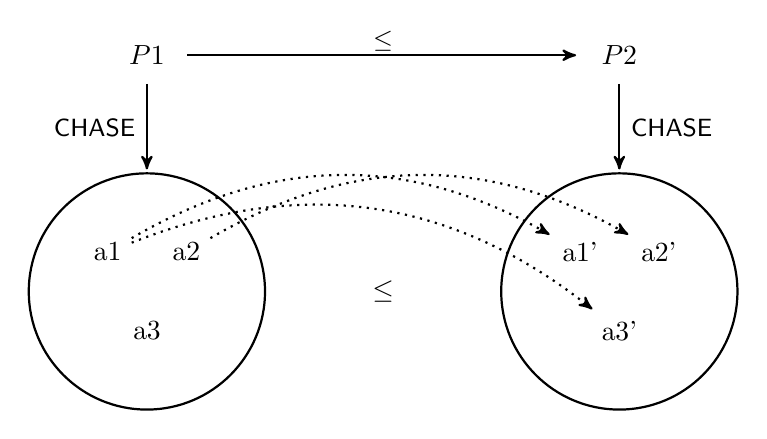
\begin{tikzpicture}[>=stealth',shorten >=1pt,auto,node distance=2.0cm,
    thick,main node/.style={rectangle,%%fill=blue!20,draw,
      font=\sffamily,minimum height=7mm,minimum width=10mm}, 
      roundnode/.style={circle, draw=black, minimum size=3cm},]
  
    \node[main node] (Phrase) {$P1$};
    %\node[main node] (ChaseP) [below of=Request] {$\langle P\rangle $};
    
    \node[main node] (Phrase') [node distance=6.0cm, right of=Phrase] {$P2$};
    % \node[main node] (ChaseP') [node distance=6.0cm, right of=Proposal] {$\langle P'\rangle$};
      
    \node[roundnode] (ChaseP) [node distance=3.0cm, below of=Phrase] {};
    \node[roundnode] (ChaseP') [node distance=6.0cm, right of=ChaseP] {};

    \node[] (a1) at (-.5,-2.5) {a1};
    \node[] (a2) at (0.5,-2.5) {a2};
    \node[] (a3) at (0,-3.5) {a3};

    \node[] (a1') at (5.5,-2.5) {a1'};
    \node[] (a2') at (6.5,-2.5) {a2'};
    \node[] (a3') at (6,-3.5) {a3'};
    %\node[] (a4') at (6.5,-3.5) {a4'};

    \node[] (ord) at (3,-3) {$\leq$};

  
    \path[every node/.style={font=\sffamily\small, fill=white,inner sep=1pt}, ->]
      (Phrase) edge node [] {$\leq$} (Phrase')
      (Phrase) edge node[left=1mm] {CHASE} (ChaseP)
      %(ChaseP) edge [dashed] node[below=1mm] {Ordering} (ChaseP')
      (Phrase') edge node[right=1mm] {CHASE} (ChaseP')
      % (a1) edge [dashed] node {} (a1')
      ;

      \draw[dotted, inner sep=0pt, ->]
        (a1) to[bend left] (a1');
      \draw[dotted, inner sep=0pt, ->]
        (a2) to[bend left] (a2');
      \draw[dotted, inner sep=0pt, ->]  
        (a1) to[bend left] (a3');
  \end{tikzpicture}
    \caption[Protocol ordering abstraction]{Diagram representing protocol ordering methodology. \\ Dashed lines represent ordering relation for individual trees holds. }
    \label{fig:protocol-org-fig}
\end{figure}

Abstractly this analysis can be visualized in Figure \ref{fig:protocol-org-fig} where solid lines represent tangible actions and dashed lines represent reasoning. Say we aim to compare two protocols $P1$ and $P2$ where we wish to determine if the change from $P1$ to $P2$ makes the protocol more difficult to attack. Recall that more difficult to attack means more difficult for an active adversary to corrupt a system while evading detection at the final measurement event of the attestation. To ascertain the relationship between the two protocols, we first run Chase to generate the set of attack trees $\{ a_1, a_2, a_3\}$ for $P1$ and the set of attack trees for $\{b_1, b_2, b_3\}$ for $P2$. We then compare the Chase-generated attack trees individually, discovering ordering relations between $a_1 \preceq b_1$, $a_2 \preceq b_2$, and $a_1 \preceq b_3$ as represented by the dotted lines with arrows pointing from an attack to one that is at least as difficult to perform. Next, looking at the sets of attack trees, we can see that every attack tree in $P2$ has a tree in $P1$ that is at most as difficult to perform. Assuming an adversary would always perform the easiest attack to thwart an appraiser, we conclude that $P2$ is at least as difficult to attack as $P1$ and thus involves at least as much adversary effort as $P1$. This logic is linked to the protocols to define $ P1 \leq P2$.  

We introduce four ordering relations for adversary-constrained protocol ordering where $=$ is an equivalence relation and $\le$ and $\ge$ are partial orders. The relations are enumerated below.

\vspace*{-5mm}

\begin{align*}
1. & \text{ } P1 = P2 \\
2. & \text{ } P1 \le P2 \\
3. & \text{ } P1 \ge P2 \\
4. & \text{ } P1 \text{ and } P2 \text{ are incomparable}
\end{align*}

\noindent We choose to define the ordering in this way for a few reasons. First, we refrain from introducing four mutually exclusive relationships (i.e., $=$, $<$, $>$, incomparable) because this results in a drastic increase in the number of incomparable protocols. As such, under our ordering, we do not conclude that one protocol is strictly better than another protocol. Although one might think we could define the relations necessary to draw such conclusions using the irreflexive kernel (deriving a strictly less than operator from the satisfaction of both less than and not equal conditions), we found this was not appropriate because the strictly less than operator would inadvertently introduce an arbitrary ordering over adversarial corruption and repair events where there should not be one.  


These four ordering relations serve as foundational categories for adversary-constrained protocol ordering. While the ordering may appear intuitive, mathematically modeling the Chase output and subsequently defining the ordering operations themselves through Coq-based mechanized proofs is challenging. Our results overcome this challenge, defining and verifying the equivalence and partial order relationships over sets of attack trees which are built upon ordering relations over individual attack trees. With this ordering infrastructure, one can provably determine that one protocol is at least as good as another because it requires at least as much adversary effort to generate seemingly trustworthy evidence. 

Under our methodology, an ordering relation between two Copland protocol can be obtained by completing the following workflow:

\begin{enumerate}
    \squash
    \item Obtain Chase output for each protocol and formally model the generated sets of attack trees
    \item Determine ordering relationships between the individual attack trees
    \item Leverage the individual ordering relationships to determine the ordering relationship between the sets of attack trees
    \item Link the set ordering relationship to determine protocol ordering relationship
\end{enumerate}

The following sections describe the process of introducing and verifying an adversary-constrained ordering between two Copland protocols. In this paper, mathematical proofs are presented manually, but mechanized versions are completed in Coq and can be found at \url{git@github.com:ku-sldg/protocol_ordering.git}.


\section{Formalized Chase Output}

This protocol ordering scheme relies on a formal model of the Chase generated attack trees. These attack trees are similar to directed, labeled graphs which contain nodes, edges, and a labeling function. 

\begin{definition}[Graph]
    A directed, labeled graph is a tuple $G = (N, E, \ell)$ where $N$ is a finite set of nodes, $E \subseteq N \times N$ is a finite set of directed edges represented as ordered pairs of nodes, and $\ell : N \rightarrow L$ is a labeling function from nodes to some set $L$ of labels. 
\end{definition}
 
An attack tree is an instance of a directed graph. Looking at Figure \ref{fig:chase-ex}, one can see that each Chase tree consists of a set of events, an arrow relationship mapping event to event, and an event labeling scheme disclosing the type of event (i.e., measurement, corruption, or repair).

\begin{definition}[Attack Tree]
    An attack tree is a directed, labeled graph where $N$ is a set of events, $E$ is a set of directed edges representing chronological time between events, and $\ell$ is a labeling function from event to measurement or adversary event label.
\end{definition}

When comparing two individual attack trees, we need only consider events that concern an active adversary. That is, it is possible for an attack tree to contain two measurement events occurring directly in sequence; the fact that two measurement events occurred instead of one does not impact the adversary. Furthermore, an attacker is not impacted by the details of any intermediate measurement events either. Instead, sequential measurement events and specific names of non-final measurement events only introduce unnecessary complications in comparing individual attack tree. Therefore, we introduce the idea of attack tree normalization, as formally defined below. Attack tree normalization reduces consecutive measurement events to a single measurement event, namely the latter one, and renames all remaining non-final measurement events to a constant label. This process results in attack trees containing only the events and information relevant to an adversary. 


\begin{definition}[Attack tree Normalization]
    An attack tree is in its normal form when all sequences of consecutive measurement events are reduced to only the final measurement event in the sequence and all remaining non-final measurement events are renamed to \texttt{ms}. 
\end{definition}

\begin{figure}[htbp]
  \centering 
  \begin{tabular}{c c}
      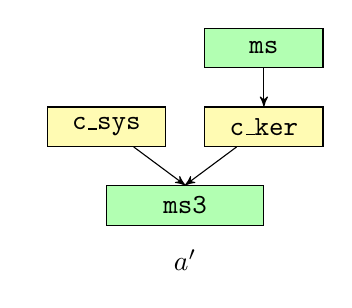
\begin{tikzpicture}[->,>=stealth']

    \node[rectangle,
          draw,
          fill = green!30,
          minimum width = 2cm, 
          minimum height = 0.5cm
          ] (ms4) at (0,0) {};
    \node[] at (ms4.center) {\texttt{ms3}};


    \node[rectangle,
        draw,
        fill = yellow!30,
        minimum width = 1.5cm, 
        minimum height = 0.5cm
        ] (sys) at (-1,1) {};
    \node[] at (sys.center) {\texttt{c\_sys}};

    \node[rectangle,
        draw,
        fill = yellow!30,
        minimum width = 1.5cm, 
        minimum height = 0.5cm
        ] (ker) at (1,1) {};
    \node[] at (ker.center) {\texttt{c\_ker}};

    \node[rectangle,
        draw,
        fill = green!30,
        minimum width = 1.5cm, 
        minimum height = 0.5cm
        ] (ms1) at (1,2) {};
    \node[] at (ms1.center) {\texttt{ms}};

    %\node[rectangle,
    %    draw,
    %    minimum width = 1.5cm, 
    %    minimum height = 0.5cm
    %    ] (ms2) at (-1,1) {};
    %\node[] at (ms2.center) {ms};

%     \node[rectangle,
%     minimum width = 1.5cm, 
%     minimum height = 0.5cm
%     ] (label) at (0,-0.5) {};
% \node[] at (label.center) {m3c};


\node[rectangle,
minimum width = 1cm, 
minimum height = 0.5cm
] (label) at (0,-.7) {};
\node[] at (label.center) {$a'$};

\node[rectangle,
minimum width = 1cm, 
minimum height = 0.5cm
] (label) at (-1.5,0) {};
\node[] at (label.center) {};


    \path[every node/.style={font=\sffamily\small}]
    %host1 path
    (ms1) edge [] node [right] {} (ker.north)
    (ker) edge [] node [right] {} (ms4.north)
    %(ms2) edge [] node [right] {} (ms4.north) 
    (sys) edge [] node [right] {} (ms4.north) ;


\end{tikzpicture} & 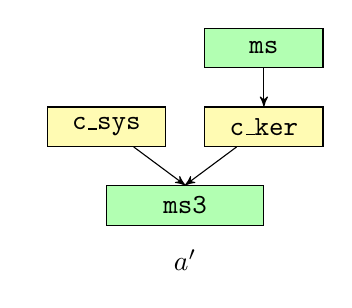
\begin{tikzpicture}[->,>=stealth']

    \node[rectangle,
          draw,
          fill = green!30,
          minimum width = 2cm, 
          minimum height = 0.5cm
          ] (ms4) at (0,0) {};
    \node[] at (ms4.center) {\texttt{ms3}};


    \node[rectangle,
        draw,
        fill = yellow!30,
        minimum width = 1.5cm, 
        minimum height = 0.5cm
        ] (sys) at (-1,1) {};
    \node[] at (sys.center) {\texttt{c\_sys}};

    \node[rectangle,
        draw,
        fill = yellow!30,
        minimum width = 1.5cm, 
        minimum height = 0.5cm
        ] (ker) at (1,1) {};
    \node[] at (ker.center) {\texttt{c\_ker}};

    \node[rectangle,
        draw,
        fill = green!30,
        minimum width = 1.5cm, 
        minimum height = 0.5cm
        ] (ms1) at (1,2) {};
    \node[] at (ms1.center) {\texttt{ms}};

    %\node[rectangle,
    %    draw,
    %    minimum width = 1.5cm, 
    %    minimum height = 0.5cm
    %    ] (ms2) at (-1,1) {};
    %\node[] at (ms2.center) {ms};

%     \node[rectangle,
%     minimum width = 1.5cm, 
%     minimum height = 0.5cm
%     ] (label) at (0,-0.5) {};
% \node[] at (label.center) {m3c};


\node[rectangle,
minimum width = 1cm, 
minimum height = 0.5cm
] (label) at (0,-.7) {};
\node[] at (label.center) {$a'$};

\node[rectangle,
minimum width = 1cm, 
minimum height = 0.5cm
] (label) at (-1.5,0) {};
\node[] at (label.center) {};


    \path[every node/.style={font=\sffamily\small}]
    %host1 path
    (ms1) edge [] node [right] {} (ker.north)
    (ker) edge [] node [right] {} (ms4.north)
    %(ms2) edge [] node [right] {} (ms4.north) 
    (sys) edge [] node [right] {} (ms4.north) ;


\end{tikzpicture} 
  \end{tabular}
  \captionsetup{justification=centering,margin=1cm}
  \caption[Example of attack tree normalization]{An example of attack tree normalization.}
  \label{fig:reduce-ex}
\end{figure}


\noindent To demonstrate attack tree normalization, consider the example presented in Figure \ref{fig:reduce-ex} where tree $a$ is normalized to $a'$. When applying attack tree normalization, the consecutive measurement events \texttt{ms2} and \texttt{ms3} are reduced to only the latter measurement event \texttt{ms2}, and the remaining non-final measurement event \texttt{ms1} is renamed to \texttt{ms}.

For the remainder of this paper, unless otherwise noted, we assume all Chase-generated attack trees are in their normal form.


\section{Ordering Individual Attack Trees}

Our main contribution lies in introducing an adversary-constrained protocol ordering through analysis of Chase-generated attack trees. Formally defined attack trees introduce necessary structures for reasoning in order to institute operations to compare attack difficulty. In the following section, we establish definitions to compare adversary events and utilize these definitions to reason over attack trees individually. Specifically, we introduce equivalence ($\simeq$), strict partial order ($\prec$), and partial order ($\preceq$) relations over individual attack trees. In future sections, these relations will be leveraged to introduce equivalence and partial order relations over sets of attack trees.

The Chase generated attack trees presented in Figure \ref{fig:chase-ex} can be used to describe the essential insights applied in developing our adversary-constrained protocol ordering. In attack tree $a$, corruption events \texttt{c\_c1} and \texttt{c\_c2} occur before any measurement events, giving the adversary a minimally-restricted amount of time to perform these actions. In attack tree $b$, corruption event \texttt{c\_c2} occurs between measurement events, confining the adversary to a small-time window to perform this action. We assert that performing the same action in a more limited time window (e.g., adversary event \texttt{c\_c2} in $b$ versus in $a$) is more challenging. Since \texttt{c\_c1} is a minimally-restricted adversary event in both $a$ and $b$, we wish to conclude that $a$ is strictly less work to perform by an adversary than $b$. Now in attack tree $c$, an adversary must perform three corruption events and one time-constrained repair event. This attack requires an adversary to perform more work than $a$ as adversary events have increased. Upon analyzing all three trees, it becomes apparent that attack $a$ presents the easiest attack given the absence of time-constrained events and the lowest number of actions required by the adversary. Because of this, we assume an adversary would perform the attack represented by tree $a$ to deceive a relying party. 

To compare individual Chase-generated attack trees, we introduce additional definitions to aid in determining when one attack tree requires strictly less or equivalent work to perform by an adversary. Central to this comparison is the different classification of adversary actions that may be present within an attack tree. That is, Chase generated attack trees contain measurement and adversary events, and it is the variety of consecutive occurences that may occur that influences our ordering definitions. 

While measurement events are self-explanatory, adversary events warrant more of an explanation and are formally defined below.
 

\begin{definition}[Adversary Event, $\pi$]
    An adversary event is any action performed by an adversary to change the behavior of a component in a target system. Adversary events are classified as either corruption or repair events. Given an attack tree $a$, let $\pi(a) := \{n \in N_a \,|\, n \text{ is an adversary event}\,\}$. An event $n$ is an adversary event if and only if $\ell_a(n)$ is an adversary event label.
\end{definition}


As previously alluded to, time constraints escalate difficulty. That is, we assume the difficulty of an attack is increased if an adversary must complete it between measurement events. To realize this distinction, we define time-constrained adversary events formally below.  

\begin{definition}[Time-Constrained Adversary Event, $\tau$]
    A time-constrained adversary event is an adversary event where the attacker must perform the corruption or repair of a component in between measurement events thus limiting the time available to complete the action. Given an attack tree $a$, let $\tau(a) := \{n \in N_a \,|\, n \text{ is a time-constrained adversary event}\,\}$.
\end{definition}

\noindent It is worth noting that by definition, every time-constrained adversary event is itself an adversary event and therefore $\tau(a) \subseteq \pi(a)$ for every attack tree $a$.


With these preliminary definitions in place, we can now describe our proposed ordering relations. We wish to say two individual attack trees are equivalent if they are semantically equivalent. Defining equivalence in this way ensures trees that have the same adversary events in the same order and the same final measurement event are indeed equivalent, regardless of the specific, intermediate measurement events that occurred. Therefore, as stated previously, we only compare trees in their normal form so that here are no sequences of consecutive measurement events and all non-final measurement events have the same label. Now we naturally define attack tree equivalence by graph isomorphism.


\begin{definition}[Isomorphism]
    Directed, labeled graphs $G$ and $H$ are isomorphic if and only if there exists a bijection $f : N_G \to N_H$ such that for all pairs of nodes $n_1, n_2 \in N_G$, $(n_1,n_2) \in E_G$ if and only if $(f(n_1),f(n_2)) \in E_H$ and for all nodes $n \in N_G$, $\ell_G(n) = \ell_H(f(n))$.
\end{definition}


\begin{definition}[Equivalence $\simeq$]
  Attack trees $a$ and $b$ are equivalent (i.e., $a \simeq b$) if and only they are isomorphic.
\end{definition}


\noindent We formally verify that an isomorphism is an equivalence relation in Coq but do not include the mathematical proofs here since they are easily available in many textbooks or web sources. With the proofs of reflexivity, symmetry, and transitivity completed in Coq, we obtain a formally-verified equivalence relation over individual attack trees allowing us to provably determine if two trees are semantically equivalent.


Next, we must define a strict partial order relation over individual attack trees. It should be the case that under this relation one attack tree is strictly better than another if it increases the burden of an attacker. To formally define the concept of increasing adversary constraint, we analyzed many Chase-generated attack trees to ground our logic in concrete examples. By studying patterns in the trees, we select two distinct conditions that confine an adversary to consider in our ordering scheme. That is, an attack has increased difficulty if it requires more adversary events or more time-constrained adversary events. We formally define this relation below as "strictly less work".

\begin{definition}[Strictly Less Work]
  An attack tree $a$ requires strictly less work to perform by an adversary than attack tree $b$ if and only if at least one of the following hold: 
\begin{enumerate}
  \squash
  \item $\pi(a) \subseteq \pi(b)$ and $\tau(a) \subset \tau(b)$
  %(i.e., the set of adversary events in $a$ is subset of the set of adversary events in $b$ and the set of time-constrained adversary events in $a$ is a proper subset of the set of time-constrained adversary events in $b$)
  \item $\pi(a) \subset \pi(b)$ and $\tau(a) \subseteq \tau(b)$
  %(i.e., the set of adversary events in $a$ is a proper subset of the set of adversary events in $b$ and the set of time-constrained adversary events in $a$ is subset of the set of time-constrained adversary events in $b$)
\end{enumerate}
\end{definition}

\noindent By design, this definition only allows the comparison of attack trees $a$ and $b$ where both $\pi(a) \subseteq \pi(b)$ and $\tau(a) \subseteq \tau(b)$. In other words, we only compare attack trees that share common sets of both adversary events and time-constrained adversary events. Looking back at Figure \ref{fig:chase-ex}, we can compute the sets of adversary events and sets of time-constrained adversary events for attacks $a$, $b$, and $c$ and then determine what ordering relationships hold between them. For attack $a$ we get that $\pi(a) = \{ \texttt{c\_c1}, \texttt{c\_c2} \}$ and $\tau(a) = \emptyset$. For attack $b$, $\pi(b) = \{ \texttt{c\_c1}, \texttt{c\_c2} \}$ and $\tau(b) = \{ \texttt{c\_c2} \}$. And lastly for attack $c$, $\pi(c) = \{ \texttt{c\_c1}, \texttt{c\_c2}, \texttt{c\_c3}, \texttt{r\_c2} \}$ and $\tau(c) = \{ \texttt{r\_c2} \}$. Using the definition of strict partial order below, we can conclude that $a \prec b$, $a \prec c$, and $b$ and $c$ are incomparable.

\begin{definition}[Strict Partial Order $\prec$]
    An attack tree $a$ is strictly less than attack tree $b$ (i.e., $a \prec b$) if and only if $a$ requires strictly less work than $b$.
\end{definition}

To formally verify this relation is indeed a strict partial order, we prove the relation is irreflexive, asymmetric, and transitive in Coq. Our proofs rely primarily on the fact that subset is a partial order and proper subset is a strict partial order. We do not present the proofs mathematically here since they are uninteresting.

We additionally define a partial order relation over individual attack trees by the combination of the equivalence and strict partial order relations defined earlier in this section. This design is motivated by the reflexive closure principle. We verify in Coq that this definition is in fact a partial order by proving it is reflexive, antisymmetric, and transitive.

\begin{definition}[Partial Order $\preceq$]
  An attack tree $a$ is less than attack tree $b$ (i.e., $a \preceq b$) if and only if $a$ is isomorphic to $b$ or $a$ requires strictly less work than $b$ (i.e., $a \simeq b$ or $a \prec b$).
\end{definition}


\section{Ordering Sets of Attack Trees}

The previously introduced ordering relations over individual attack trees can be leveraged to compare protocols by ordering their corresponding sets of Chase-generated attack trees. 

First, we naturally define an equivalence relation over sets of attack trees using set equality up to isomorphism. This means that when determining one set is a subset of another, instead of requiring every element in the former to be in the latter, we only require every element in the former to be isomorphic/equivalent to an element in the latter. Mathematically, we replace the representation of $S \subseteq T$ from $\forall s \in S, s \in T$ to $\forall s \in S, \exists t \in T, s \simeq t$.

\begin{definition}[Set Equality]
  Two sets $S$ and $T$ are equal if and only $S \subseteq T$ and $T \subseteq S$.
\end{definition}

\begin{definition}[Equivalence =]
    Two sets of attack trees $S$ and $T$ are equivalent (i.e., $S = T$) if and only if they are equal up to isomorphism of their elements.
\end{definition}

Now before we can introduce a partial order relation, we must introduce additional infrastructure to compare sets of attack trees. We begin by recalling Rowe's definition of supports and covers below \cite{Rowe:2021:OnOrdering}.

\begin{definition}[Supports/Covers]
    Given two sets of graphs $S$ and $T$ and some preorder $R$ over graphs, we say that $S$ supports $T$ if and only if for every $h \in T$, there is some $g \in S$, such that $R\: g\: h$. We  say that $T$ covers $S$ if and only if for every $g \in S$ there is some $h \in T$ such that $R\: g\: h$.
\end{definition}

Supports states that, for every tree in $T$, there exists some related tree in $S$. Conversely, covers says that, for every tree in $S$, there exists a related tree in $T$.  This idea is best visualized by Figure \ref{fig:sup-cov} where we abstractly denote Copland protocols as $S$ and $T$. We assume these protocols generate the corresponding sets of attack trees $\{a1, a2 , a3 \}$ and $ \{b1, b2 ,b3\}$.

\begin{figure}[htbp]
    \centering
    \usetikzlibrary{shapes.geometric}

\begin{tikzpicture}


    \node[ellipse,
    draw = black,
    minimum width = 1.5cm, 
    minimum height = 3cm] (e) at (-4.8,0) {};

    \node[ellipse,
    draw = black,
    minimum width = 1.5cm, 
    minimum height = 3cm] (e) at (-1.8,0) {};

    \node[ellipse,
    draw = black,
    minimum width = 1.5cm, 
    minimum height = 3cm] (e) at (1.8,0) {};

    \node[ellipse,
    draw = black,
    minimum width = 1.5cm, 
    minimum height = 3cm] (e) at (4.8,0) {};


    \node[] (a1) at (-4.8,.8) {$a_1$};
    \node[] (a2) at (-4.8,0) {$a_2$};
    \node[] (a3) at (-4.8,-.8) {$a_3$};

    \node[] (a1') at (-1.8,.8) {$b_1$};
    \node[] (a2') at (-1.8,0) {$b_2$};
    \node[] (a3') at (-1.8,-.8) {$b_3$};

    \node[] (b1) at (4.8,.8) {$b_1$};
    \node[] (b2) at (4.8,0) {$b_2$};
    \node[] (b3) at (4.8,-.8) {$b_3$};

    \node[] (b1') at (1.8,.8) {$a_1$};
    \node[] (b2') at (1.8,0) {$a_2$};
    \node[] (b3') at (1.8,-.8) {$a_3$};

    \node[] (label) at (-3.3, -2.1) {$S$ supports $T$};
    \node[] (label) at (3.3, -2.1) {$T$ covers $S$};

    \node[] (label) at (-4.8, 1.9) {$S$};
    \node[] (label) at (-1.8, 1.9) {$T$};

    \node[] (label) at (1.8, 1.9) {$S$};
    \node[] (label) at (4.8, 1.9) {$T$};


      \draw[->] (a1) to (a1');
      \draw[->] (a2) to (a2');
      \draw[->] (a2) to (a3');

      \draw[->] (b1') to (b1);
      \draw[->] (b2') to (b1);
      \draw[->] (b3') to (b1);
  \end{tikzpicture}
    \captionsetup{justification=centering,margin=1cm}
    \caption[Supports and covers]{A visual representation of supports and covers. \\ Arrows represent ordering relationships.}
    \label{fig:sup-cov}
\end{figure}

The definition of supports and covers is parameterized over a relation $R$. For an adversary-constrained protocol ordering, we choose $R$ to be the partial order over attack trees defined previously. Therefore, in Figure \ref{fig:sup-cov}, arrows between the individual attack trees represent partial order relationships.

While Rowe defines both supports and covers, we only need to be concerned with supports for our adversary-constrained protocol ordering. The motivation for this two-fold. First, we assume that given a protocol and its associated attacks, an adversary will always perform the easiest one (i.e., some attack $a$ such that $\forall b \in S, b \npreceq a$ where $S$ is the associated set of attack trees). Second, we must consider our desired conclusion of protocol ordering: if a protocol $S$ is less than a protocol $T$, then $T$ is at least as good as $S$ and therefore \emph{should be selected over $S$}. Therefore, we must consider every attack in the better protocol so as not to overlook the easiest attack. Furthermore, we need not consider every tree in the weaker protocol. This is best understood by examining the two extreme cases for the skipped tree: it is the easiest attack, or it is the hardest attack. If it is the easiest attack, then clearly the protocol is still the weaker one. If it is the hardest attack, then it has no effect on the protocol since, by our assumption, an attacker would not choose this attack.

\begin{definition}[Partial Order $\leq$]
  A set of attack trees $S$ is less than a set of attack trees $T$ (i.e., $S \leq T$) if and only if S supports T with the partial order relation $\preceq$.
\end{definition} 

Recall that a partial order is reflexive, antisymmetric, and transitive. We easily verify in Coq that our proposed partial order relation is reflexive and transitive. Verifying that the relation is antisymmetric proved more difficult and, in fact, impossible. That is, it is impossible using the classic definition of antisymmetry (i.e., if $S \le T$ and $T \le S$ then $S = T$). A simple counter example can be constructed using the attack trees in Figure \ref{fig:chase-ex}. Let $S = \{a,b\}$ and $T = \{a\}$. Then $S \le T$ since $a \preceq a$, and $T \le S$ since $a \preceq a$ and $a \preceq b$. But clearly it is not the case that $S$ is the same set as $T$. Instead, we can see that set of weakest attacks in $S$ is the same set as the set of weakest attacks in $T$. In fact, this property holds not only for this example but for any two protocols. Therefore, we construct and prove a modified version of antisymmetry. Before we give its precise specification, we must provide a preliminary definition.

\begin{definition}[Minimal Attack Tree, \normalfont{min}]
  An attack tree $a$ is minimal with respect to a set $S$ if and only $b \nprec a$ for every $b \in S$. Given a set of attack trees $S$, let $min(S) := \{a \in S \,|\, a \text{ is minimal with respect to } S \}$.
\end{definition}

Our revised version of antisymmetry is stated as follows: if $S \le T$ and $T \le S$ then min($S$) = min($T$). Although this property is mathematically weaker than its standard version, it is, in practice, considering our goals, adequately and equally as strong.

%% Talk about proof of antisymmetry

With verified equivalence and partial order relations, we can link the ordering decision over sets of attack trees to their corresponding protocols allows us to provably state that one protocol is at least as difficult to attack as another protocol. If no ordering relation holds, the protocols are incomparable. Therefore, with the additional definitions for individual attack tree comparison and set comparison, we have formally verified the four previously defined mutually inclusive relationships hold for ordering Copland protocols. By leveraging existing tools, like the Chase model finder, we were able to successfully capture all possible attacks and adversary may launch yet go undetected. This ordering reasons over those attacks, successfully introducing a proven adversary-constrained protocol ordering. 


\section{Representative Examples}

This research finds inspiration in real-life instances of Copland protocol analysis documented in the attestation literature \cite{Rowe:2021:OnOrdering,Coker::Principles-of-R}. We ground our formally-verified adversary-constrained protocol ordering model in reality by reasoning about a relying party who would like to ensure a remote server (target) is free of viruses. Taken from Rowe's \cite{Rowe:2016:Confining} example, the target's infrastructure consists of two platforms $P3$ and $P4$ which depend on a hardware root of trust (rtm). Additionally, within $P4$, the system $sys$ is dependent on the virus checker $vc$ which is dependent on the kernel $ker$.  Each platform has various measurement operations (ASPs), including a virus checking measurement and a kernel integrity measurement. From this system, we derive possible Copland protocols and perform various manipulations of their structure and order. We then apply previously derived formal reasoning to determine the most adversary-constrained protocol, further establishing correctness in our model.

%Taken from Rowe's \cite{Rowe:2016:Confining} example, the target's infrastructure is abstractly rendered in Figure \ref{fig:ord-system}. In this system, there are two platforms $P3$ and $P4$ which depend on a hardware root of trust (rtm). Additional system dependencies within $P4$ are denoted with dashed lines.  Each platform has various measurement operations (ASPs), including a virus checking measurement $vc$ and a kernel integrity measurement $ker$. From this system, we derive possible Copland protocols and perform various manipulations of their structure and order. We then apply previously derived formal reasoning to determine the most adversary-constrained protocol, further establishing correctness in our model.

% \begin{figure}[htbp]
%     \centering
%     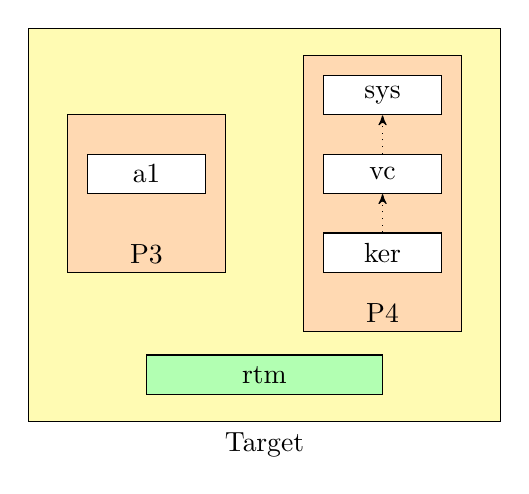
\begin{tikzpicture}[->,>=stealth']

    %\node (req) at (-6,0) {Request, *P0};

    \node[rectangle,
          draw,
          fill = yellow!30,
          minimum width = 6cm, 
          minimum height = 5cm] (r) at (0,-.4) {};
    \node[anchor=north] at (r.south) {Target};
    
    \node[rectangle,
          draw,
          fill = orange!30,
          minimum width = 2cm, 
          minimum height = 2cm] (AM) at (-1.5,0) {};
    \node[anchor=south] at (AM.south) {P3}; 

    \node[rectangle,
          draw,
          fill = white,
          minimum width = 1.5cm, 
          minimum height = 0.5cm] (ASP) at (-1.5,0.25) {};
    \node at (ASP.center) {a1};

    \node[rectangle,
          draw,
          fill = orange!30,
          minimum width = 2cm, 
          minimum height = 3.5cm] (Host2) at (1.5,0) {};
    \node[anchor=south] at (Host2.south) {P4}; 

    \node[rectangle,
          draw,
          fill = white,
          minimum width = 1.5cm, 
          minimum height = 0.5cm] (sys) at (1.5,1.25) {};
    \node at (sys.center) {sys};
    

    \node[rectangle,
    draw,
    fill = white,
    minimum width = 1.5cm, 
    minimum height = .5cm] (vc) at (1.5,0.25) {};
    \node at (vc.center) {vc};

    \node[rectangle,
    draw,
    fill = white,
    minimum width = 1.5cm, 
    minimum height = .5cm] (ker) at (1.5,-0.75) {};
    \node at (ker.center) {ker};

    \node[rectangle,
    draw,
    fill = green!30,
    minimum width = 3cm, 
    minimum height = 0.5cm] (RoTM) at (0,-2.3) {};
    \node at (RoTM.center) {rtm};



    \path[every node/.style={font=\sffamily\small}]
    %host1 path
%    (req) edge node [right] {} (r.west)
%     (ASP.east) edge[draw=red,dotted] node [left] {} (sys.west)
%     % host2 path
     (vc.north) edge [dotted] node [left] {} (sys.south)
     (ker.north) edge [dotted] node {} (vc.south);
%     (RoTM.north) edge [dotted] node {} (ker.south) ;

\end{tikzpicture}
%     \captionsetup{justification=centering,margin=1cm}
%     \caption[Example system for protocol ordering]{Example system for protocol ordering motivated by \cite{Rowe:2016:Confining}.\\ Dashed lines represent dependencies. }
%     \label{fig:ord-system}
% \end{figure}

Within the forthcoming protocol ordering examples, we assume that the adversary has manipulated the system and somehow allowed the resulting evidence to appear trustworthy when it is not. We also assume the root of trust (rtm) is inherently trusted and therefore cannot be attacked. We explicitly state these assumptions and the system's dependency structure in the Chase input files.

We introduce three distinct scenarios to investigate the impact of adversary constraint when manipulating measurement operations and measurement composition. In the first example, we test the effects of well-supported measurements on an attacker's difficulty of attack. In the second and third examples, we test various effects of protocol composition. Each experiment is tested under our formally defined adversary-constrained model to assign one of the four relationships.

The first example hypothesizes that creating a more comprehensive protocol, one where targets and their dependencies are measured, produces more trustworthy evidence. This hypothesis was initially validated manually, relying on intuition and logical reasoning \cite{Rowe:2016:Confining}. To test this hypothesis under our formal model, we selected the following three protocols presented in Table \ref{Chase-table} where again the goal of each measurement is to ascertain if a system is free from viruses. The Copland phrase that accomplishes this is $\at{p4}{(vc\; p4\; sys)}$. This measurement is therefore the final phrase in each protocol. By maintaining the same final measurement event, we focus our investigation towards the effect of adversary constraint on protocol comprehensiveness.


\begin{table}[htbp]
    \setlength\extrarowheight{7pt}
    \centering
    \footnotesize
    \begin{tabular}{|M{3cm}|M{7cm}|N}
        \hline
        Protocol Name & Actual protocol &\\
        \hline
        sys & *target: $\at{p4}{(vc\; p4\; sys)}$  &\\ 
        %\hline
        % a1-vc-sys-seq & *target: $\at{p3}{[(a1\; p4\; vc) \braseqe\pi \at{p4}{(vc\; p4\; sys)}]}$ &\\ 
        \hline   
        ker-vc-sys-seq & *target:  $\at{p4}{[(ker\; p4\; vc)}$ \texttt{+<+} $\at{p4}{(vc\; p4\; sys)}]$ &\\ \hline 
        rtm-ker-vc-sys-seq & *target: $\at{p1}{[(rtm\; p4\; ker)}$ \texttt{+<+} $\at{p4}{[(ker\; p4\; vc)}$ \texttt{+<+} $\at{p4}{(vc\; p4\; sys)}]]$ &\\
        \hline
    \end{tabular}
    \caption[Chase Analysis with Varied Dependencies]{Sequential protocols analyzed with Chase, mimicking layered measurement style}
    \label{Chase-table}
\end{table}

When constructing this case study, we start from the simplest protocol and sequentially prepend measurement operations until reaching a root of trust, carefully crafting each protocol to mimic the system's dependencies. The first protocol, \texttt{sys}, is a measurement of the system using the virus checker. If the virus checking ASP is inadvertently corrupted, the resulting evidence will lack validity. To ensure the trustworthiness of the virus checking ASP, one may utilize one of the virus checking dependencies to measure the virus checker prior to its measurement of the system. This is achieved through the \texttt{ker-vc-sys-seq} protocol, where the kernel ASP \emph{ker} is invoked to measure the virus checker \emph{vc} before the virus checker \emph{vc} measures the system \emph{sys}. By measuring within the dependency chain, we hypothetically strengthen the resulting evidence. Taking this reasoning a step further, the protocol \texttt{rtm-ker-vc-sys-seq} includes a prepended measurement of the kernel \emph{ker}, performed by the root of trust $rtm$, prior to $ker$'s measurement of the virus checker. Because the root of trust is a trusted source, we can hypothetically further strengthen the resulting evidence. 

\setlength{\textfloatsep}{0.1cm}
\begin{figure}[hbtp]
    \begin{center}
        \begin{tabular}{ M{3.6cm} | M{4.1cm} | M{4.1cm} }
                sys & ker-vc-sys-seq & rtm-ker-vc-sys-seq \\
                \hline
                &&\\ \input{examples/sys/sys1.tex} & \input{examples/ker_vs-sys-seq_reduced/m1.tex} & \input{examples/rtm_ker-vc-sys-seq_reduced/m1.tex} \\ 
                m1a & m1b & m1c \\ 
                &&\\
                \begin{tikzpicture}[->,>=stealth']

    \node[rectangle,
          draw,
          fill = green!30,
          minimum width = 2cm, 
          minimum height = 0.5cm
          ] (ms4) at (0,0) {};
    \node[] at (ms4.center) {\texttt{ms4}};


    \node[rectangle,
        draw,
        fill = yellow!30,
        minimum width = 1.5cm, 
        minimum height = 0.5cm
        ] (sys) at (-1,1) {};
    \node[] at (sys.center) {\texttt{c\_sys}};

    \node[rectangle,
        draw,
        fill = yellow!30,
        minimum width = 1.5cm, 
        minimum height = 0.5cm
        ] (ker) at (1,1) {};
    \node[] at (ker.center) {\texttt{c\_ker}};

    \node[rectangle,
        minimum width = 1.5cm, 
        minimum height = 0.5cm
        ] (ms3) at (1,2) {};
    \node[] at (ms3.center) {};


    % \node[rectangle,
    %     minimum width = 1cm, 
    %     minimum height = 0.5cm
    %     ] (label) at (0,-1) {};
    % \node[] at (label.center) {m2a};


    \path[every node/.style={font=\sffamily\small}]
    %host1 path
    (vc) edge [] node [right] {} (ms4.north) 
    (sys) edge [] node [right] {} (ms4.north) ;


\end{tikzpicture} & 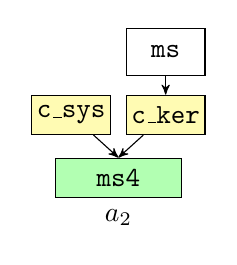
\begin{tikzpicture}[->,>=stealth']

    \node[rectangle,
          draw,
          fill = green!30,
          minimum width = 1.6cm, 
          minimum height = 0.5cm
          ] (ms4) at (0,0) {};
    \node[] at (ms4.center) {\texttt{ms4}};

    \node[rectangle,
    minimum width = 1cm, 
    minimum height = 0.5cm
    ] (lab) at (0,-.5) {};
  \node[] at (lab.center) {$a_2$};

    \node[rectangle,
        draw,
        fill = yellow!30,
        minimum width = 1cm, 
        minimum height = 0.5cm
        ] (sys) at (-.6,.8) {};
    \node[] at (sys.center) {\texttt{c\_sys}};

    \node[rectangle,
        draw,
        fill = yellow!30,
        minimum width = 1cm, 
        minimum height = 0.5cm
        ] (vc) at (.6,.8) {};
    \node[] at (vc.center) {\texttt{c\_ker}};

    \node[rectangle,
        draw,
        minimum width = 1cm, 
        minimum height = 0.6cm
        ] (ms3) at (.6,1.6) {};
    \node[] at (ms3.center) {\texttt{ms}};

%     \node[rectangle,
%     minimum width = 1cm, 
%     minimum height = 0.5cm
%     ] (label) at (0,-0.5) {};
% \node[] at (label.center) {m2b};


    \path[every node/.style={font=\sffamily\small}]
    %host1 path
    (ms3) edge [] node [right] {} (vc.north)
    (vc) edge [] node [right] {} (ms4.north) 
    (sys) edge [] node [right] {} (ms4.north) ;


\end{tikzpicture} & 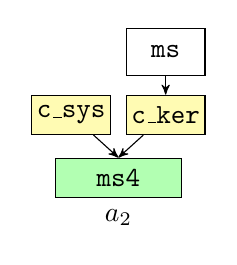
\begin{tikzpicture}[->,>=stealth']

    \node[rectangle,
          draw,
          fill = green!30,
          minimum width = 1.6cm, 
          minimum height = 0.5cm
          ] (ms4) at (0,0) {};
    \node[] at (ms4.center) {\texttt{ms4}};

    \node[rectangle,
    minimum width = 1cm, 
    minimum height = 0.5cm
    ] (lab) at (0,-.5) {};
  \node[] at (lab.center) {$a_2$};

    \node[rectangle,
        draw,
        fill = yellow!30,
        minimum width = 1cm, 
        minimum height = 0.5cm
        ] (sys) at (-.6,.8) {};
    \node[] at (sys.center) {\texttt{c\_sys}};

    \node[rectangle,
        draw,
        fill = yellow!30,
        minimum width = 1cm, 
        minimum height = 0.5cm
        ] (vc) at (.6,.8) {};
    \node[] at (vc.center) {\texttt{c\_ker}};

    \node[rectangle,
        draw,
        minimum width = 1cm, 
        minimum height = 0.6cm
        ] (ms3) at (.6,1.6) {};
    \node[] at (ms3.center) {\texttt{ms}};

%     \node[rectangle,
%     minimum width = 1cm, 
%     minimum height = 0.5cm
%     ] (label) at (0,-0.5) {};
% \node[] at (label.center) {m2b};


    \path[every node/.style={font=\sffamily\small}]
    %host1 path
    (ms3) edge [] node [right] {} (vc.north)
    (vc) edge [] node [right] {} (ms4.north) 
    (sys) edge [] node [right] {} (ms4.north) ;


\end{tikzpicture}  \\   
                m2a & m2b & m2c \\ 
                &&\\
                & \input{examples/ker_vs-sys-seq_reduced/m3.tex}  & \input{examples/rtm_ker-vc-sys-seq_reduced/m3.tex} \\  
                  & m3b & m3c \\ 
                 &&\\ 
                  & 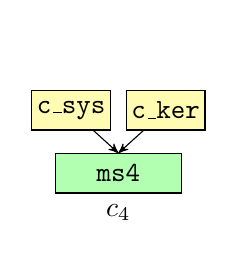
\begin{tikzpicture}[->,>=stealth']

  \node[rectangle,
        draw,
        fill = green!30,
        minimum width = 1.6cm, 
        minimum height = 0.5cm
        ] (ms4) at (0,0) {};
  \node[] at (ms4.center) {\texttt{ms4}};

  \node[rectangle,
  minimum width = 1cm, 
  minimum height = 0.5cm
  ] (lab) at (0,-.5) {};
\node[] at (lab.center) {$c_4$};

  %\node[rectangle,
  %    draw,
  %    minimum width = 1.5cm, 
  %    minimum height = 0.5cm
  %    ] (ms) at (-1,1) {};
  %\node[] at (ms.center) {ms};

  \node[rectangle,
      draw,
      fill = yellow!30,
      minimum width = 1cm, 
      minimum height = 0.5cm
      ] (ker) at (.6,.8) {};
  \node[] at (ker.center) {\texttt{c\_ker}};

  \node[rectangle,
      draw,
      fill = yellow!30,
      minimum width = 1cm, 
      minimum height = 0.5cm
      ] (sys) at (-.6,.8) {};
  \node[] at (sys.center) {\texttt{c\_sys}};

  \node[rectangle,
      minimum width = 1cm, 
      minimum height = 0.5cm
      ] (ms3) at (.6,1.6) {};
  \node[] at (ms3.center) {};

%     \node[rectangle,
%     minimum width = 1cm, 
%     minimum height = 0.5cm
%     ] (label) at (0,-0.5) {};
% \node[] at (label.center) {m3b};


  \path[every node/.style={font=\sffamily\small}]
  %host1 path
  (ker) edge [] node [right] {} (ms4.north)
  (sys) edge [] node [right] {} (ms4.north) ;
  % (ms) edge [] node [right] {} (ms4.north) ;


\end{tikzpicture} & 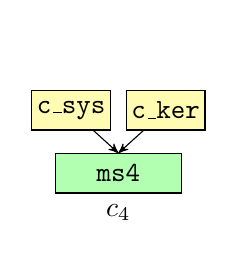
\begin{tikzpicture}[->,>=stealth']

  \node[rectangle,
        draw,
        fill = green!30,
        minimum width = 1.6cm, 
        minimum height = 0.5cm
        ] (ms4) at (0,0) {};
  \node[] at (ms4.center) {\texttt{ms4}};

  \node[rectangle,
  minimum width = 1cm, 
  minimum height = 0.5cm
  ] (lab) at (0,-.5) {};
\node[] at (lab.center) {$c_4$};

  %\node[rectangle,
  %    draw,
  %    minimum width = 1.5cm, 
  %    minimum height = 0.5cm
  %    ] (ms) at (-1,1) {};
  %\node[] at (ms.center) {ms};

  \node[rectangle,
      draw,
      fill = yellow!30,
      minimum width = 1cm, 
      minimum height = 0.5cm
      ] (ker) at (.6,.8) {};
  \node[] at (ker.center) {\texttt{c\_ker}};

  \node[rectangle,
      draw,
      fill = yellow!30,
      minimum width = 1cm, 
      minimum height = 0.5cm
      ] (sys) at (-.6,.8) {};
  \node[] at (sys.center) {\texttt{c\_sys}};

  \node[rectangle,
      minimum width = 1cm, 
      minimum height = 0.5cm
      ] (ms3) at (.6,1.6) {};
  \node[] at (ms3.center) {};

%     \node[rectangle,
%     minimum width = 1cm, 
%     minimum height = 0.5cm
%     ] (label) at (0,-0.5) {};
% \node[] at (label.center) {m3b};


  \path[every node/.style={font=\sffamily\small}]
  %host1 path
  (ker) edge [] node [right] {} (ms4.north)
  (sys) edge [] node [right] {} (ms4.north) ;
  % (ms) edge [] node [right] {} (ms4.north) ;


\end{tikzpicture}  \\
                 & m4b & m4c \\ 
                &&\\  
                 & 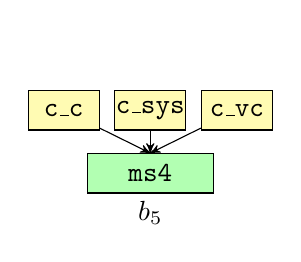
\begin{tikzpicture}[->,>=stealth']

    \node[rectangle,
          draw,
          fill = green!30,
          minimum width = 1.6cm, 
          minimum height = 0.5cm
          ] (ms4) at (0,0) {};
    \node[] at (ms4.center) {\texttt{ms4}};

    \node[rectangle,
    minimum width = 1cm, 
    minimum height = 0.5cm
    ] (lab) at (0,-.5) {};
  \node[] at (lab.center) {$b_5$};

    \node[rectangle,
        draw,
        fill = yellow!30,
        minimum width = .9cm, 
        minimum height = 0.5cm
        ] (vc) at (1.1,.8) {};
    \node[] at (vc.center) {\texttt{c\_vc}};

    \node[rectangle,
        draw,
        fill = yellow!30,
        minimum width = .9cm, 
        minimum height = 0.5cm
        ] (c) at (-1.1,.8) {};
    \node[] at (c.center) {\texttt{c\_c}};

    \node[rectangle,
        draw,
        fill = yellow!30,
        minimum width = .9cm, 
        minimum height = 0.5cm
        ] (sys) at (0,.8) {};
    \node[] at (sys.center) {\texttt{c\_sys}};

    \node[rectangle,
        minimum width = .9cm, 
        minimum height = 0.5cm
        ] (ms3) at (1.1,1.6) {};
    \node[] at (ms3.center) {};


    \path[every node/.style={font=\sffamily\small}]
    %host1 path
    (vc) edge [] node [right] {} (ms4.north)
    (c) edge [] node [right] {} (ms4.north)
    (sys) edge [] node [right] {} (ms4.north) ;
    % (ms) edge [] node [right] {} (ms4.north) ;


\end{tikzpicture} & 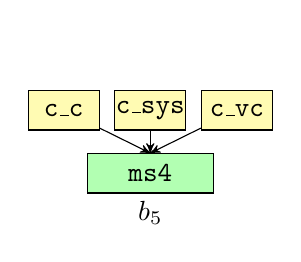
\begin{tikzpicture}[->,>=stealth']

    \node[rectangle,
          draw,
          fill = green!30,
          minimum width = 1.6cm, 
          minimum height = 0.5cm
          ] (ms4) at (0,0) {};
    \node[] at (ms4.center) {\texttt{ms4}};

    \node[rectangle,
    minimum width = 1cm, 
    minimum height = 0.5cm
    ] (lab) at (0,-.5) {};
  \node[] at (lab.center) {$b_5$};

    \node[rectangle,
        draw,
        fill = yellow!30,
        minimum width = .9cm, 
        minimum height = 0.5cm
        ] (vc) at (1.1,.8) {};
    \node[] at (vc.center) {\texttt{c\_vc}};

    \node[rectangle,
        draw,
        fill = yellow!30,
        minimum width = .9cm, 
        minimum height = 0.5cm
        ] (c) at (-1.1,.8) {};
    \node[] at (c.center) {\texttt{c\_c}};

    \node[rectangle,
        draw,
        fill = yellow!30,
        minimum width = .9cm, 
        minimum height = 0.5cm
        ] (sys) at (0,.8) {};
    \node[] at (sys.center) {\texttt{c\_sys}};

    \node[rectangle,
        minimum width = .9cm, 
        minimum height = 0.5cm
        ] (ms3) at (1.1,1.6) {};
    \node[] at (ms3.center) {};


    \path[every node/.style={font=\sffamily\small}]
    %host1 path
    (vc) edge [] node [right] {} (ms4.north)
    (c) edge [] node [right] {} (ms4.north)
    (sys) edge [] node [right] {} (ms4.north) ;
    % (ms) edge [] node [right] {} (ms4.north) ;


\end{tikzpicture}   \\
                 & m5b & m5c \\ 
                &&\\
            \end{tabular}
    \end{center}
    \caption{Normalized attack trees for sys, ker-vc-sys-seq, and rtm-ker-vc-sys-seq}
    \label{fig:rtm-compare-reduced}
\end{figure}

% Employing the previously introduced formalism, it becomes possible to demonstrate that \emph{rtm-ker-vc-sys-seq} is indeed the most resistant to attacks, establishing it as the optimal protocol. 

Formal reasoning to demonstrate that \emph{rtm-ker-vc-sys-seq} is indeed the most resistant to attacks begins by obtaining the Chase generated attack trees for each protocol. With the protocols presented in Table \ref{Chase-table} and the necessary Chase inputs, we obtain the following attack models presented in Figure \ref{fig:rtm-compare}. After applying tree normalization, the attack trees can be reduced to only activities that affect an active adversary, as presented in Figure \ref{fig:rtm-compare-reduced}.  The remainder of this analysis will only consider the trees under normal form. 



Employing the previously introduced formalism to determine the relationship between the three protocols begins by analyzing the underlying relationship between individual attack trees. Starting with \texttt{m1a}, it is apparent that \texttt{m1b} is strictly better than \texttt{m1a} because \texttt{m1b} has a time-constrained measurement event. The same logic applies when comparing \texttt{m2a} and \texttt{m2b}. It is also apparent that tree \texttt{m3b} is equivalent to \texttt{m2a} because they have the same corruption events. \texttt{m4b} is strictly better than either \texttt{m2a} or \texttt{m1a} because it has more corruption events. By the same reasoning, \texttt{m5b} is strictly better than \texttt{m1a}. This concludes comparison of the individual attack trees.

Next, we apply the supports formalism to determine the relationship between the sets of attack trees. Because every tree generated by \texttt{ker-vc-sys-seq} requires the adversary to apply either the same effort or more effort to attack when compared to \texttt{sys}, we say that \texttt{ker-vc-sys-seq} is at least as adversary constrained as \texttt{sys}. Said differently, we find that \texttt{ker-vc-sys-seq} supports \texttt{sys}, as denoted with the following relationship: sys $\leq$ ker-vs-sys-seq.

We apply the same logic to compare \texttt{ker-vc-sys-seq} and \texttt{rtm-ker-vc-sys-seq}. That is, we first compare the protocols' individual Chase-generated attack trees. Again, looking at the reduced trees in Figure \ref{fig:rtm-compare-reduced}, we see that  \texttt{m1c} and  \texttt{m1b} are the same tree; they are equivalent under the bidirectional homomorphism. \texttt{m2c} and \texttt{m2b} are also the same tree thus equivalent. \texttt{m3c} has more time-constrained corruption events when compared to  \texttt{m3b} thus  \texttt{m3c} is strictly better than \texttt{m3b}. The same logic applies to \texttt{m4c} and  \texttt{m4b} where  \texttt{m4b} is strictly less than  \texttt{m4c} because  \texttt{m4c} has more time-constrained corruption events.  \texttt{m5c} and \texttt{m5b} are equivalent. Propagating the findings of individual attack tree comparisons and considering the formalism of supports, we conclude that \texttt{ker-vc-sys-seq} is less than or equal to \texttt{rtm-ker-vc-sys-seq} because every tree in \texttt{rtm-ker-vc-sys-seq} requires the adversary to perform equal or more effort to attack when compared to every tree in  \texttt{ker-vc-sys-seq}. 

Ultimately, we arrive at the ordering below. Formal analysis therefore supports our hypothesis that a measurement which considers system dependencies up to a root of trust, is more difficult to attack and therefore better constrains the adversary. 
\begin{center}
    sys $\leq$ ker-vc-sys-seq $\leq$ rtm-ker-vc-sys-seq
\end{center}

%% next example is measuring from a different place 
Secondly, we investigate the impact of measurement location on adversary constraint specifically studying the effects of attacks when all measurements are carried out on the same platform compared to a separate platform. To test this hypothesis, the following protocols presented in Table \ref{Chase-table-location} were analyzed with Chase and subsequently subjected to the ordering methodology. The baseline protocol \texttt{sys} calls the virus checker located on \texttt{p4} to measure the system \texttt{sys}. The next protocol \texttt{ker-vc-sys-seq} calls the kernel ASP \emph{ker} to measure the virus checker $vc$ prior to the \texttt{sys} measurement. It is important to note that the kernel ASP is located on the same platform, $P4$, as \emph{vc} and \emph{sys}. Again, we know from the system description, that the system depends on the virus checker and the virus checker depends on the kernel. In the third protocol, \texttt{a1-vc-sys-seq}, the ASP \emph{a1}, located on a separate platform \emph{p3}, is used to measure the virus checker prior to the \texttt{sys} measurement. \emph{a1} is not included in the dependency chain of \emph{vc} or \emph{sys} but simply another attestation capability within the target system.

% \begin{table}[htbp]
%     \setlength\extrarowheight{7pt}
%     \centering
%     \begin{tabular}{|M{4cm}|M{10cm}|N}
%     \hline
%         Protocol Name & Actual protocol &\\
%     \hline
%         sys & *target: $\at{p4}{(vc\; p4\; sys)}$  &\\ 
%     \hline   
%         ker-vc-sys-seq & *target:  $\at{p4}{[(ker\; p4\; vc)}$ \texttt{+<+} $\at{p4}{(vc\; p4\; sys)}]$ &\\ 
%     \hline
%      a1-vc-sys-seq & *target: $\at{p3}{[(a1\; p4\; vc)}$ \texttt{+<+} $\at{p4}{(vc\; p4\; sys)}]$ &\\ \hline 
%     \end{tabular}
%     \caption[Chase Analysis with Varied Place]{Protocols analyzed regarding location of prior measurements with Chase}
%     \label{Chase-table-location}
% \end{table}

% \begin{figure}[hbtp]
%     %\setlength\extrarowheight{20pt}
%     \begin{center}
%         % \begin{tabular}{ M{3.75cm} | M{5cm} | M{5cm}}
%         \begin{tabular}{ c | c | c}
%         sys & ker-vc-sys-seq & a1-vc-sys-seq \\
%         \hline
%         &&\\
%         \input{examples/sys/sys1.tex} & \input{examples/ker_vs-sys-seq_reduced/m1.tex} & \input{examples/a1-vc-sys-seq/vc-sys-seq1.tex}  \\ 
%         m1a & m1b & m1c \\ 
%         &&\\
%         \begin{tikzpicture}[->,>=stealth']

    \node[rectangle,
          draw,
          fill = green!30,
          minimum width = 2cm, 
          minimum height = 0.5cm
          ] (ms4) at (0,0) {};
    \node[] at (ms4.center) {\texttt{ms4}};


    \node[rectangle,
        draw,
        fill = yellow!30,
        minimum width = 1.5cm, 
        minimum height = 0.5cm
        ] (sys) at (-1,1) {};
    \node[] at (sys.center) {\texttt{c\_sys}};

    \node[rectangle,
        draw,
        fill = yellow!30,
        minimum width = 1.5cm, 
        minimum height = 0.5cm
        ] (ker) at (1,1) {};
    \node[] at (ker.center) {\texttt{c\_ker}};

    \node[rectangle,
        minimum width = 1.5cm, 
        minimum height = 0.5cm
        ] (ms3) at (1,2) {};
    \node[] at (ms3.center) {};


    % \node[rectangle,
    %     minimum width = 1cm, 
    %     minimum height = 0.5cm
    %     ] (label) at (0,-1) {};
    % \node[] at (label.center) {m2a};


    \path[every node/.style={font=\sffamily\small}]
    %host1 path
    (vc) edge [] node [right] {} (ms4.north) 
    (sys) edge [] node [right] {} (ms4.north) ;


\end{tikzpicture} & 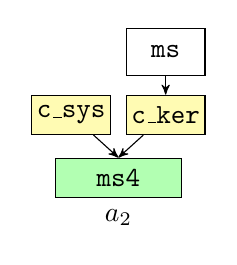
\begin{tikzpicture}[->,>=stealth']

    \node[rectangle,
          draw,
          fill = green!30,
          minimum width = 1.6cm, 
          minimum height = 0.5cm
          ] (ms4) at (0,0) {};
    \node[] at (ms4.center) {\texttt{ms4}};

    \node[rectangle,
    minimum width = 1cm, 
    minimum height = 0.5cm
    ] (lab) at (0,-.5) {};
  \node[] at (lab.center) {$a_2$};

    \node[rectangle,
        draw,
        fill = yellow!30,
        minimum width = 1cm, 
        minimum height = 0.5cm
        ] (sys) at (-.6,.8) {};
    \node[] at (sys.center) {\texttt{c\_sys}};

    \node[rectangle,
        draw,
        fill = yellow!30,
        minimum width = 1cm, 
        minimum height = 0.5cm
        ] (vc) at (.6,.8) {};
    \node[] at (vc.center) {\texttt{c\_ker}};

    \node[rectangle,
        draw,
        minimum width = 1cm, 
        minimum height = 0.6cm
        ] (ms3) at (.6,1.6) {};
    \node[] at (ms3.center) {\texttt{ms}};

%     \node[rectangle,
%     minimum width = 1cm, 
%     minimum height = 0.5cm
%     ] (label) at (0,-0.5) {};
% \node[] at (label.center) {m2b};


    \path[every node/.style={font=\sffamily\small}]
    %host1 path
    (ms3) edge [] node [right] {} (vc.north)
    (vc) edge [] node [right] {} (ms4.north) 
    (sys) edge [] node [right] {} (ms4.north) ;


\end{tikzpicture} & \input{examples/a1-vc-sys-seq/vc-sys-seq2.tex}  \\ 
%         m2a & m2b & m2c \\
%         &&\\    & \input{examples/ker_vs-sys-seq_reduced/m3.tex} & \input{examples/a1-vc-sys-seq/vc-sys-seq3.tex}  \\ 
%             & m3b & m3c \\
%         &&\\  & 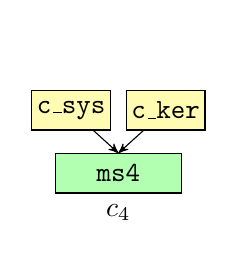
\begin{tikzpicture}[->,>=stealth']

  \node[rectangle,
        draw,
        fill = green!30,
        minimum width = 1.6cm, 
        minimum height = 0.5cm
        ] (ms4) at (0,0) {};
  \node[] at (ms4.center) {\texttt{ms4}};

  \node[rectangle,
  minimum width = 1cm, 
  minimum height = 0.5cm
  ] (lab) at (0,-.5) {};
\node[] at (lab.center) {$c_4$};

  %\node[rectangle,
  %    draw,
  %    minimum width = 1.5cm, 
  %    minimum height = 0.5cm
  %    ] (ms) at (-1,1) {};
  %\node[] at (ms.center) {ms};

  \node[rectangle,
      draw,
      fill = yellow!30,
      minimum width = 1cm, 
      minimum height = 0.5cm
      ] (ker) at (.6,.8) {};
  \node[] at (ker.center) {\texttt{c\_ker}};

  \node[rectangle,
      draw,
      fill = yellow!30,
      minimum width = 1cm, 
      minimum height = 0.5cm
      ] (sys) at (-.6,.8) {};
  \node[] at (sys.center) {\texttt{c\_sys}};

  \node[rectangle,
      minimum width = 1cm, 
      minimum height = 0.5cm
      ] (ms3) at (.6,1.6) {};
  \node[] at (ms3.center) {};

%     \node[rectangle,
%     minimum width = 1cm, 
%     minimum height = 0.5cm
%     ] (label) at (0,-0.5) {};
% \node[] at (label.center) {m3b};


  \path[every node/.style={font=\sffamily\small}]
  %host1 path
  (ker) edge [] node [right] {} (ms4.north)
  (sys) edge [] node [right] {} (ms4.north) ;
  % (ms) edge [] node [right] {} (ms4.north) ;


\end{tikzpicture} & \input{examples/a1-vc-sys-seq/vc-sys-seq4.tex}  \\ 
%         & m4b & m4c \\
%         &&\\ & 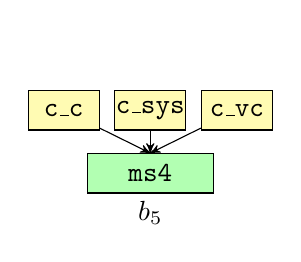
\begin{tikzpicture}[->,>=stealth']

    \node[rectangle,
          draw,
          fill = green!30,
          minimum width = 1.6cm, 
          minimum height = 0.5cm
          ] (ms4) at (0,0) {};
    \node[] at (ms4.center) {\texttt{ms4}};

    \node[rectangle,
    minimum width = 1cm, 
    minimum height = 0.5cm
    ] (lab) at (0,-.5) {};
  \node[] at (lab.center) {$b_5$};

    \node[rectangle,
        draw,
        fill = yellow!30,
        minimum width = .9cm, 
        minimum height = 0.5cm
        ] (vc) at (1.1,.8) {};
    \node[] at (vc.center) {\texttt{c\_vc}};

    \node[rectangle,
        draw,
        fill = yellow!30,
        minimum width = .9cm, 
        minimum height = 0.5cm
        ] (c) at (-1.1,.8) {};
    \node[] at (c.center) {\texttt{c\_c}};

    \node[rectangle,
        draw,
        fill = yellow!30,
        minimum width = .9cm, 
        minimum height = 0.5cm
        ] (sys) at (0,.8) {};
    \node[] at (sys.center) {\texttt{c\_sys}};

    \node[rectangle,
        minimum width = .9cm, 
        minimum height = 0.5cm
        ] (ms3) at (1.1,1.6) {};
    \node[] at (ms3.center) {};


    \path[every node/.style={font=\sffamily\small}]
    %host1 path
    (vc) edge [] node [right] {} (ms4.north)
    (c) edge [] node [right] {} (ms4.north)
    (sys) edge [] node [right] {} (ms4.north) ;
    % (ms) edge [] node [right] {} (ms4.north) ;


\end{tikzpicture} & \\
%         & m5b &  \\
%         \end{tabular}
%     \end{center}
%     \caption{Reduced attack trees for sys, ker-vc-sys-seq, and a1-vc-sys-seq}
%     \label{fig:chase-location}
% \end{figure}

One may hypothesize that \texttt{ker-vc-sys-seq} is the strongest measurement because it includes measurements within the system's dependency chain. However, the generated Chase models, presented in Figure \ref{fig:chase-location} in their normal form, did not support this hypothesis. When first analyzing the trees, it is apparent that both protocols \texttt{ker-vc-sys-seq} and \texttt{a1-vc-sys-seq} are at least as good as \texttt{sys}. This claim holds because all attack trees in the more detailed protocols are the same or require more effort than the attack trees generated by \texttt{sys}. However, when comparing \texttt{ker-vc-sys-seq} and \texttt{a1-vc-sys-seq} the relationship is harder to recognize. For instance, consider the tree \texttt{m4b}. It is more difficult to attack when compared to \texttt{m1a} or \texttt{m2a} because it has more corruption events. However, there is not a relatable tree in \texttt{a1-vc-sys-seq} because there is no tree that includes corruption events of \emph{vc}, \emph{ker}, and \emph{sys}. A similar Chase generated model may be \texttt{m3c} or \texttt{m4c}, but adversary events do not have the same label. Therefore, we must conclude that  \texttt{ker-vc-sys-seq} and \texttt{a1-vc-sys-seq} are incomparable. This may actually be desired behavior because we cannot make claims about the difficulty of a specific attack. 


%% third example for ordering 
The third facet of protocol ordering investigates the impact of Copland protocol composition, sequential versus parallel, on adversary capability. \citet{Rowe:2021:AutomatedTrust} motivates the use of Chase to compare attack difficultly, manually studying specific examples with sequential measurements that mimic the system's dependency structure versus parallel measurements with no specified order. \citet{Rowe:2021:AutomatedTrust} logically deduced sequential measurements would better constrain the adversary because measuring within the system's dependency structure would require more complex attacks. We set out to apply our mathematical model to this hypothesis, testing the effects of protocol composition over the target system in Figure \ref{fig:ord-system}. 

In Table \ref{Chase-table-order}, we present three protocols where the latter two have varied composition. The first protocol, \texttt{sys}, is a baseline measurement. The next two protocols include an additional measurement involving the kernel $ker$ measuring the virus checker $vc$. The difference between the two measurements is the composition. In \texttt{ker-vc-sys-seq}, the measurements are performed in sequence. In \texttt{ker-vc-sys-par}, measurements are performed in parallel. By altering the composition dynamics in these protocols, we are able to investigate the effects on adversary constraint.

% \begin{table}[htbp]
%     \setlength\extrarowheight{7pt}
%     \centering
%     \begin{tabular}{|M{4cm}|M{10cm}|N}
%     \hline
%         Protocol Name & Actual protocol &\\
%     \hline
%         sys & *target: $\at{p4}{(vc\; p4\; sys)}$  &\\ 
%     \hline
%     ker-vc-sys-seq & *target:  $\at{p4}{[(ker\; p4\; vc)}$ \texttt{+<+} $\at{p4}{(vc\; p4\; sys)}]$ &\\ \hline 
%     ker-vc-sys-par & *target: $\at{p3}{[(ker\; p4\; vc)}$ \texttt{+}$\sim$\texttt{+} $\at{p4}{(vc\; p4\; sys)}]$ &\\ 
%         \hline   
%     \end{tabular}
%     \caption[Chase Analysis with Varied Composition]{Protocols analyzed regarding measurement composition with Chase}
%     \label{Chase-table-order}
% \end{table}

%Beyond the protocol input incorporating diverse composition operators, we maintain consistency in utilizing identical files for the Chase input to ensure accurate analysis. 
Executing Chase with the three distinct protocols yields the normalized attack trees presented in Figure \ref{fig:chase-comp-trees} where protocol ordering methodology yields incomparable results between the sequential and parallel protocols. Upon analyzing these trees, it becomes evident that the inclusion of additional measurement operations -- specifically those mirroring the dependency chain -- more effectively constrains an adversary. This observation arises from the comparison of \texttt{sys} with both \texttt{ker-vc-sys-seq} and \texttt{ker-vc-sys-par}, wherein both of the latter protocols support \texttt{sys}. When evaluating the relationship between \texttt{ker-vc-sys-seq} and \texttt{ker-vc-sys-par}, determining which one supports the other is not obvious. Notably, trees \texttt{m2b} and \texttt{m2c} are identical and therefore equal. Similarly, \texttt{m1c} and \texttt{m3b} involve the same attacks and culminate in the same final measurement event, so they are equivalent. The complexity arises when comparing \texttt{m3c} to other attack trees. While \texttt{m3c} is more difficult to attack than \texttt{m2a} due to the additional adversary (repair) event, comparing it with any tree generated by \texttt{ker-vc-sys-par} in its current form is impossible. Since the final measurement event of \texttt{m3c} differs from that in any tree generated by \texttt{ker-vc-sys-par} and the repair event cannot be found in any tree generated by \texttt{ker-vc-sys-par}, we find that \texttt{ker-vc-sys-seq} and \texttt{ker-vc-sys-par} are incomparable. This contradicts the conclusions presented by \citet{Rowe:2021:AutomatedTrust}. 

% \begin{figure}
% \begin{center}
% \begin{tabular}{ c |  c | c }
%     sys & ker-vc-sys-seq & ker-vc-sys-par  \\
%     \hline
%     &&\\
%     \input{examples/sys/sys1.tex} & \input{examples/ker_vs-sys-seq_reduced/m1.tex} & \input{examples/vc-sys-par/m1'.tex} \\
%     m1a & m1b & m1c \\ 
%     &&\\
%     \begin{tikzpicture}[->,>=stealth']

    \node[rectangle,
          draw,
          fill = green!30,
          minimum width = 2cm, 
          minimum height = 0.5cm
          ] (ms4) at (0,0) {};
    \node[] at (ms4.center) {\texttt{ms4}};


    \node[rectangle,
        draw,
        fill = yellow!30,
        minimum width = 1.5cm, 
        minimum height = 0.5cm
        ] (sys) at (-1,1) {};
    \node[] at (sys.center) {\texttt{c\_sys}};

    \node[rectangle,
        draw,
        fill = yellow!30,
        minimum width = 1.5cm, 
        minimum height = 0.5cm
        ] (ker) at (1,1) {};
    \node[] at (ker.center) {\texttt{c\_ker}};

    \node[rectangle,
        minimum width = 1.5cm, 
        minimum height = 0.5cm
        ] (ms3) at (1,2) {};
    \node[] at (ms3.center) {};


    % \node[rectangle,
    %     minimum width = 1cm, 
    %     minimum height = 0.5cm
    %     ] (label) at (0,-1) {};
    % \node[] at (label.center) {m2a};


    \path[every node/.style={font=\sffamily\small}]
    %host1 path
    (vc) edge [] node [right] {} (ms4.north) 
    (sys) edge [] node [right] {} (ms4.north) ;


\end{tikzpicture} & 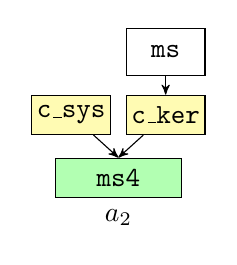
\begin{tikzpicture}[->,>=stealth']

    \node[rectangle,
          draw,
          fill = green!30,
          minimum width = 1.6cm, 
          minimum height = 0.5cm
          ] (ms4) at (0,0) {};
    \node[] at (ms4.center) {\texttt{ms4}};

    \node[rectangle,
    minimum width = 1cm, 
    minimum height = 0.5cm
    ] (lab) at (0,-.5) {};
  \node[] at (lab.center) {$a_2$};

    \node[rectangle,
        draw,
        fill = yellow!30,
        minimum width = 1cm, 
        minimum height = 0.5cm
        ] (sys) at (-.6,.8) {};
    \node[] at (sys.center) {\texttt{c\_sys}};

    \node[rectangle,
        draw,
        fill = yellow!30,
        minimum width = 1cm, 
        minimum height = 0.5cm
        ] (vc) at (.6,.8) {};
    \node[] at (vc.center) {\texttt{c\_ker}};

    \node[rectangle,
        draw,
        minimum width = 1cm, 
        minimum height = 0.6cm
        ] (ms3) at (.6,1.6) {};
    \node[] at (ms3.center) {\texttt{ms}};

%     \node[rectangle,
%     minimum width = 1cm, 
%     minimum height = 0.5cm
%     ] (label) at (0,-0.5) {};
% \node[] at (label.center) {m2b};


    \path[every node/.style={font=\sffamily\small}]
    %host1 path
    (ms3) edge [] node [right] {} (vc.north)
    (vc) edge [] node [right] {} (ms4.north) 
    (sys) edge [] node [right] {} (ms4.north) ;


\end{tikzpicture} & \input{examples/vc-sys-par/m2'.tex} \\
%     m2a & m2b & m2c \\ 
%     &&\\
%     & \input{examples/ker_vs-sys-seq_reduced/m3.tex} & \input{examples/vc-sys-par/m3'.tex} \\ 
%     & m3b & m3c \\ 
%     &&\\
%     & 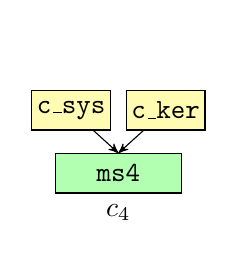
\begin{tikzpicture}[->,>=stealth']

  \node[rectangle,
        draw,
        fill = green!30,
        minimum width = 1.6cm, 
        minimum height = 0.5cm
        ] (ms4) at (0,0) {};
  \node[] at (ms4.center) {\texttt{ms4}};

  \node[rectangle,
  minimum width = 1cm, 
  minimum height = 0.5cm
  ] (lab) at (0,-.5) {};
\node[] at (lab.center) {$c_4$};

  %\node[rectangle,
  %    draw,
  %    minimum width = 1.5cm, 
  %    minimum height = 0.5cm
  %    ] (ms) at (-1,1) {};
  %\node[] at (ms.center) {ms};

  \node[rectangle,
      draw,
      fill = yellow!30,
      minimum width = 1cm, 
      minimum height = 0.5cm
      ] (ker) at (.6,.8) {};
  \node[] at (ker.center) {\texttt{c\_ker}};

  \node[rectangle,
      draw,
      fill = yellow!30,
      minimum width = 1cm, 
      minimum height = 0.5cm
      ] (sys) at (-.6,.8) {};
  \node[] at (sys.center) {\texttt{c\_sys}};

  \node[rectangle,
      minimum width = 1cm, 
      minimum height = 0.5cm
      ] (ms3) at (.6,1.6) {};
  \node[] at (ms3.center) {};

%     \node[rectangle,
%     minimum width = 1cm, 
%     minimum height = 0.5cm
%     ] (label) at (0,-0.5) {};
% \node[] at (label.center) {m3b};


  \path[every node/.style={font=\sffamily\small}]
  %host1 path
  (ker) edge [] node [right] {} (ms4.north)
  (sys) edge [] node [right] {} (ms4.north) ;
  % (ms) edge [] node [right] {} (ms4.north) ;


\end{tikzpicture} &  \\
%     & m4b & \\ 
%     &&\\    
% \end{tabular}
% \end{center}
% \caption{Reduced attack trees for \texttt{ker-vc-sys-seq} and \texttt{ker-vc-sys-par}}
% \label{fig:chase-comp-trees}
% \end{figure}

An intriguing nuance emerging from studying protocol compositions is the frequent occurrence of attack trees with repair events in the Chase output of Copland phrases with parallel measurement operations. It is common to find instances where parallel measurements, mimicking the dependency chain, are not executed in an order that replicates the dependencies. Consequently, the Chase analysis often includes trees where, at the top level measurement, the adversary corrupts a component but then must subsequently repair it before it undergoes measurement. This scenario precisely unfolds in tree m3c: the virus checker is corrupted, leading to a measurement of a compromised system, but repair becomes necessary before the virus checker itself is measured.

This observation prompts us to consider the effort involved in a repair event. That is, if an adversary already has a foothold in the system through a previously corrupted component, how challenging is it for them to repair that same component? The difficulty of this decision is context-dependent and lies within the judgment of an informed analyst. If informed attestation analyst determines that the effort required for the repair event in tree \texttt{m3c} is minimal, then perhaps tree \texttt{m3c} is equivalent to tree \texttt{m2a} or strictly less than tree \texttt{m2a}. Following this order, \texttt{ker-vc-sys-seq} supports both \texttt{ker-vc-sys-par} and \texttt{sys}, leading us to conclude that \texttt{ker-vc-sys-seq} is the most difficult to attack and therefore the best protocol. This conclusion would align with the intuition presented by \citet{Rowe:2021:AutomatedTrust}.

%\subsubsection*{Summary}

These examples demonstrate the applicability of this ordering approach to examples from the literature. With these completed examples, we reliably conclude our adversary-constrained protocol ordering methodology successfully enhances the evaluation of remote attestation protocols. Leveraging the Chase model finder, we order Copland protocols according to their adversary constraint by comparing all possible attack trees and linking the relationship between attack trees to the protocol in question. By testing various protocol composition and protocol ordering hypotheses regarding Copland phrases, we reliably conclude that measuring according to the system's dependency chain provably increases the trustworthiness of generated evidence. This methodology introduces a novel approach to protocol ordering, paving the way for more complex examples to ultimately create more robust and resilient attestation systems.



%%%%%%%%%%%
% Quick and dirty example using \verb+listings+ to format Coq code:

% \begin{lstlisting}[language=coq]
%   Definition x:nat := 3.
%   Fixpoint f(x:nat):nat := if x=0 then 1 else x*f(x-1).
% \end{lstlisting}

%
% 
% ---- Bibliography ----
%
% BibTeX users should specify bibliography style 'splncs04'.
% References will then be sorted and formatted in the correct style.
%
%\bibliographystyle{splncs04}
\bibliographystyle{splncsnat}
%\bibliography{sldg}
\bibliography{works}
%
\end{document}
